\documentclass{beamer}
\usepackage[T1]{fontenc}
\usepackage[utf8]{inputenc}
%\usepackage{natbib}
\usepackage{bibentry}

\usepackage[francais]{babel}
\usepackage{graphicx}
\usepackage{geometry}
\usepackage{eurosym}


\usepackage{comment}

\bibliographystyle{plain}


\graphicspath{{./Figures/}{./Animations/}}

\mode<presentation> {
	\usetheme{Singapore}
	%\usetheme{Madrid}
}



\def\onedot{$\mathsurround0pt\ldotp$}
\def\cddot{% two dots stacked vertically
	\mathbin{\vcenter{\baselineskip.67ex
			\hbox{\onedot}\hbox{\onedot}}%
}}



\newcommand{\matr}[1]{\bm{#1}} 

\newcommand{\blue}[1]{\textcolor{blue}{#1}}
\newcommand{\red}[1]{\textcolor{red}{#1}}
\newcommand{\green}[1]{\textcolor{red}{#1}}

% make bibliography entries smaller
%\renewcommand\bibfont{\scriptsize}
% If you have more than one page of references, you want to tell beamer
% to put the continuation section label from the second slide onwards
%\setbeamertemplate{frametitle continuation}[from second]
% Now get rid of all the colours
%\setbeamercolor*{bibliography entry title}{fg=black}
%\setbeamercolor*{bibliography entry author}{fg=black}
%\setbeamercolor*{bibliography entry location}{fg=black}
%\setbeamercolor*{bibliography entry note}{fg=black}
% and kill the abominable icon
%\setbeamertemplate{bibliography item}{}


\expandafter\def\expandafter\insertshorttitle\expandafter{%
	\insertshorttitle\hfill%
	\insertframenumber\,/\,\inserttotalframenumber}


\title[Collaboration avec l'ITA]{Presentation du projet de collaboration avec l'ITA \\ (Istituto Tecn\'ologico de Aeron\'autica)}
\author[A. Brugnoli ISAE-SUPAERO]{\small Andrea Brugnoli \\
 \footnotesize Directeurs des Theses: Daniel Alazard (ISAE-SUPAERO), Valerie Pommer-Budinger (ISAE-SUPAERO) \\
\footnotesize Encadrant à l'ITA: Flavio Luiz Cardoso Riberio}
%\date{23 janvier 2014}

% Clear the navigation bar
\setbeamertemplate{navigation symbols}{}
%\setbeamercolor{section in head/foot}{fg=black, bg=white} 




%\AtBeginSection[]
%{
%	\begin{frame}<beamer>
%	\frametitle{Outline}
%	\tableofcontents[sectionstyle=show/shaded, subsectionstyle=show/show/hide]
%\end{frame}
%}

%\AtBeginSubsection[]
%{
%\begin{frame}<beamer>
%\frametitle{Outline}
%\tableofcontents[sectionstyle=show/shaded, subsectionstyle=show/shaded/hide]
%\end{frame}
%}



\begin{document}
	
	
	
\begin{frame}
	\titlepage
\begin{columns}
	\begin{column}{0.5\textwidth}
		\centering
		\includegraphics[height=0.2\textheight]{ISAE-SUPAERO.png}
	\end{column}
	\begin{column}{0.5\textwidth}
		\centering
		\includegraphics[scale=0.3]{ITA_logo.png}
	\end{column}
\end{columns}

\end{frame}

\begin{frame}
\frametitle{Sujet de Thèse}
"Modélisation et Contrôle par le formalisme pHs des structures flexibles 2D avec des conditions aux limites variantes".\\
\vspace{5mm}
Le formalisme PH compte plusieurs avantages:
\begin{itemize}
\item approche modulaire à la modélisation des systèmes multi-physique permettant de garder la même structure de base;
\item l'énergie est au centre de la modélisation et cela permet de implémenter de lois de commande simple pour garantir la passivité et la stabilité;

\end{itemize}
Par exemple un peu imaginer de modéliser un satellite avec plusieurs panneaux solaires:

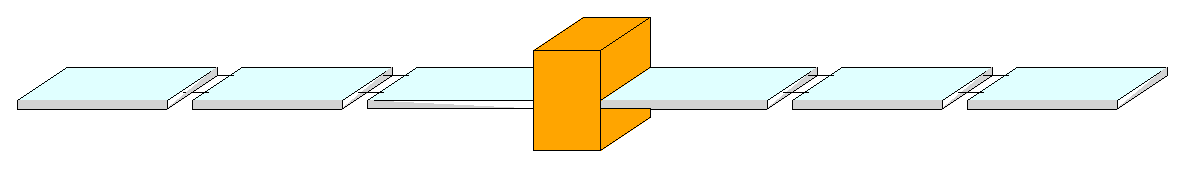
\includegraphics[width=0.99 \columnwidth]{multiarray.eps}
\end{frame}

\begin{frame}

\frametitle{Publications}
\nobibliography*
\bibentry{BrugnoliMin} \\
\vspace{3mm}
\bibentry{BrugnoliKir}
\end{frame}



\begin{frame}
\frametitle{La laboratoire d'accueil}
\begin{itemize}
\item Laboratoire: Laborat\'orio de Novos Conceitos en aeron\'autica;
\item Professeur Correspondant: Fl\'avio Luiz Cardoso-Riberio;
\end{itemize}
Flavio à soutenu sa thèse en 2016 sous la direction de Denis Matignon et Valérie Budinger. Son travail à démontré l'efficacité de l'approche Port-Hamiltonien grâce à l'utilisation un banc expérimental.  

\footnotesize
\bibentry{LHMNLCFlavio2018} \\
\vspace{3mm}
\bibentry{articleFlavio}
\end{frame}

\begin{frame}
\frametitle{Directions de Recherche}
Thématiques principales :
\begin{itemize}
\item contrôle optimal pour systèmes distribués;
\item réduction de modèle;
\item applications dans le domaine spatial;
\end{itemize}
Pour la partie recherche on se propose d'introduire les concepts de commande optimale dans le formalisme port Hamiltonien. Avant tout il faudra réduire la taille des modèle générés par la méthodes des éléments finis.
\end{frame}

\begin{frame}
\frametitle{Budget}

\begin{tabular}{|c|c|c|}
	\hline 
\textbf{Dépense}	& \textbf{Co\^uts} & \textbf{Financement} \\ 
	\hline 
Voyage AR Toulouse Sau Paulo	& 1500 \euro  & ED-ISAE \\ 
	\hline 
 Logement (4 mois)	& 1500 \euro & Laboratoire (DCAS) \\ 
	\hline 
Transports sur place & 500 \euro  & \textcolor{blue}{EDSYS} \\ 
	\hline
Assurances, visa, frais de change... & 500 \euro  & \textcolor{blue}{EDSYS} \\ 
\hline
\textbf{Total}	& \textbf{4000} \euro &  \\ 
	\hline 
\end{tabular} 

\end{frame}




\end{document}